\documentclass[spanish]{beamer}
\usepackage[utf8]{inputenc}
\usepackage{float}
\usepackage{beamerthemesplit}
\usepackage{latexsym}
\usepackage[T1]{fontenc}
\usepackage{amsmath}
\usepackage{hyperref}
\usepackage{graphicx}
\usepackage{babel,blindtext}
\usepackage{amsfonts}
\usepackage[round]{natbib}
\bibliographystyle{chicago}
\usepackage{subcaption} 


\decimalpoint

\usetheme{Madrid}%este es el templete que se usa a lo largo de la presentacion
%themes
%   default
%   Boadilla
%   Madrid
%   Pittsburgh
%   Copenhagen
%   Warsaw
%   Singapore
%   Malmoe
\newcommand\Fontvi{\fontsize{6}{7.2}\selectfont}
\mode<presentation>%tipo de 
\begin{document}

%%%%%%%%%%%%%%%%%%%%%%%%%%%%%%%%%%%%%%%%%%%%%%%%%%%%%%%%%%%%%%%%%%%%%%%%%%%%%%%%%%%%%%%%%%%%%%%%%%%%%%%%%%%%%
\title{Regresión lineal por gradiente descendente}
\author{Gamaliel Moreno Chávez}
\institute{MCPI}
\date{Evaluación\\ 2021}%para que ponga la fecha de hoy 

\frame{\titlepage}
%%%%%%%%%%%%%%%%%%%%%%%%%%%%%%%%%%%%%%%%%%%%%%%%%%%%%%%%%%%%%%%%%%%%%%%%%%%%%%%%%%%%%%%%%%%%%%%%%%%%%%%%%%%%%
%%%%%%%%%%%%%%%%%%%%%%%%%%%%%%%%%%%%%%%%%%%%%%%%%%%%%%%%%%%%%%%%%%%%%%%%%%%%%%%%%%%%%%%%%%%%%%%%%%%%%%%%%%%%%%%%%%%%%%%%%%%%%%%%%%%%%%%%%%%%%%%%%%%%%%%%%%%%%%%%%%%%%%%%%%%%%%%%%%%%%%%%%%%%%%%%%%%%%%%%%%%%%%%%%%%%%%%%%%
%%%%%%%%%%%%%%%%%%%%%%%%%%%%%%%%%%%%%%%%%%%%%%%%%%%%%%%%%%%%%%%%%%%%%%%%%%%%%%%%%%%%%%%%%%%%%%%%%%%%%%%%%%%%%%%%%%%%%%%%%%%%%%%%%%%%%%%%%%%%%%%%%%%%%%%%%%%%%%%%%%%%%%%%%%%%%%%%%%%%%%%%%%%%%%%%%%%%%%%%%%%%%%%%%%%%%%%%%%

\begin{frame}
\frametitle{Contenido}
\begin{itemize}
\item Aprendizaje supervisado
\item Regresión lineal 
\item Descenso por gradiente
\end{itemize}
\end{frame}
%%%%%%%%%%%%%%%%%%%%%%%%%%%%%%%%%%%%%%%%%%%%%%%%%%%%%%%%%%%%%%%%%%%%%%%%%%%%%%%%%%%%%%%%%%%%%%%%%%%%%%%%%%%%%

\begin{frame}
\frametitle{Aprendizaje supervisado}
Aprendizaje supervisado. métodos entrenados con:

\begin{itemize}
\item Conjunto de entrenamiento con pares ordenados $(\mathbf{x}^{(i)},y^{(i)})$
\item $\mathbf{x}^{(i)}$ es el i-ésimo vector de entrada 
\item $y^{(i)}$ es la correspondiente etiqueta (label) correcta que se desea predecir posteriormente
\item Descenso por gradiente
\end{itemize}

Es el tipo de aprendizaje más común.
\end{frame}


%%%%%%%%%%%%%%%%%%%%%%%%%%%%%%%%%%%%%%%%%%%%%%%%%%%%%%%%%%%%%%%%%%%%%%%%%%%%%%%%%%%%%%%%%%%%%%%%%%%%%%%%%%%%%


\begin{frame}
\frametitle{Problema}
 
Dado un conjunto de entrenamiento como el que se muestra en la figura, ¿Cómo se puede encontrar la relación de salida en términos de la entrada?
\begin{columns}
\begin{column}{0.3\textwidth}
\begin{center}
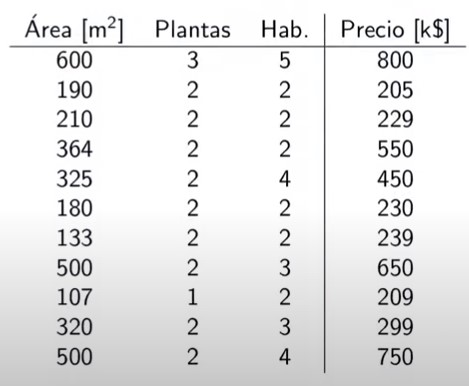
\includegraphics[scale=0.4]{imb}
\end{center}

\end{column}
\begin{column}{0.7\textwidth}
\begin{center}
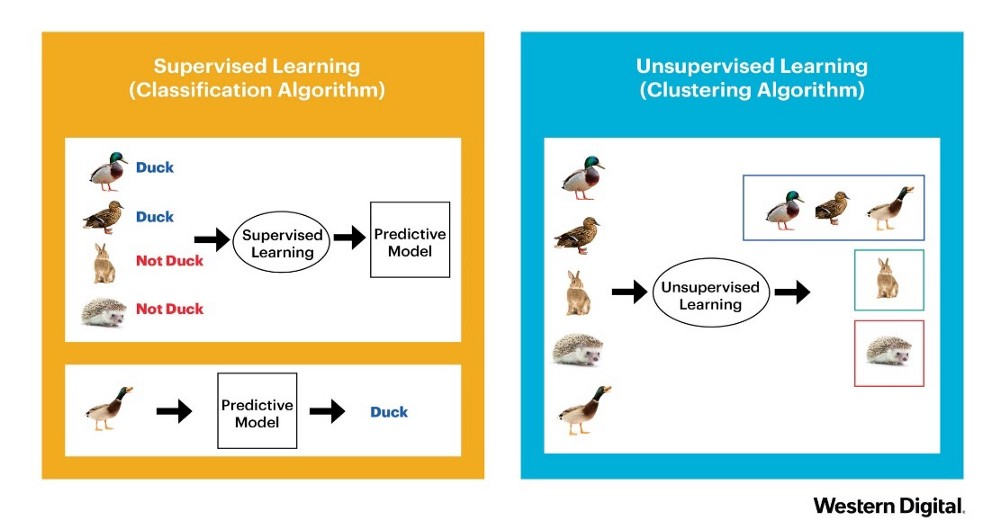
\includegraphics[scale=0.4]{im1}
\end{center}
\end{column}
\end{columns}
\end{frame}


%%%%%%%%%%%%%%%%%%%%%%%%%%%%%%%%%%%%%%%%%%%%%%%%%%%%%%%%%%%%%%%%%%%%%%%%%%%%%%%%%%%%%%%%%%%%%%%%%%%%%%%%%%%%%


\begin{frame}
\frametitle{Notación y modelo supervisado}

\begin{columns}
\begin{column}{0.3\textwidth}
\begin{center}
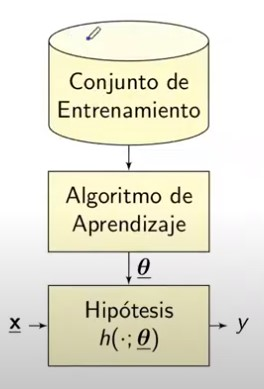
\includegraphics[scale=0.5]{im2}
\end{center}
\end{column}
\begin{column}{0.7\textwidth}
\begin{itemize}
\item $m$: números de muestras de entrenamiento 
\item $\mathbf{x}$: datos de entrada 
\item $n$ : dimensión de la entrada  $\mathbf{x}$ (número de características)
\item $y$: variable de salida u objetivo (target)
 \begin{itemize}
\item Clasificación: $y \in \lbrace C_{1},\ldots , C_{k}\rbrace k\in \mathbb{N}$
\item Regresión: $ y \in \mathbb{R}$  

\end{itemize} 
\item $(\mathbf{x}^{(i)},y^{(i)})$: i-ésima muestra de entrenamiento 
\item $\boldsymbol{\theta}:$ parámetros 
\item $y=h(\mathbf{x};\boldsymbol{\theta})$: hipótesis
\end{itemize}
\end{column}
\end{columns}

\end{frame}


%%%%%%%%%%%%%%%%%%%%%%%%%%%%%%%%%%%%%%%%%%%%%%%%%%%%%%%%%%%%%%%%%%%%%%%%%%%%%%%%%%%%%%%%%%%%%%%%%%%%%%%%%%%%%

\begin{frame}
\frametitle{Hipótesis para regresión lineal}
\begin{itemize}
\item Ejemplo de hipótesis: regresión lineal 
\begin{equation*}
y=h(\mathbf{x}; \boldsymbol{\theta})= h_{\boldsymbol{\theta}}(\mathbf{x})= \theta_0+\theta_1x_1+\cdots + \theta_n x_n
\end{equation*}
\item Ejemplo con n=3 
\begin{itemize}
\item $x_{1}$: área de casa 
\item $x_{2}$: \# de habitaciones 
\item $x_{3}$: \# de pisos 
\end{itemize} 
\item Convención para simplificar notación: $x_0={1}$
\begin{equation*}
y=h(\mathbf{x}; \boldsymbol{\theta})= h_{\boldsymbol{\theta}}(\mathbf{x})= \theta_0x_0+\theta_1x_1+\cdots + \theta_n x_n=\sum_{i=0}^{n}{\theta_{i}x_{i}}
\end{equation*} 
\begin{equation*}
=\boldsymbol{\theta}^T  \mathbf{x}= \langle \boldsymbol{\theta},  \mathbf{x} \rangle= \boldsymbol{\theta} \cdot{}  \mathbf{x}
\end{equation*}
\begin{equation*}
\boldsymbol{\theta} = [\theta_{0},\theta_{1}, \ldots ,\theta_{n}]^T
\end{equation*}  
\begin{equation*}
\boldsymbol{x} = [x_{0},x_{1}, \ldots ,x_{n}]^T
\end{equation*}  
\end{itemize}


\end{frame}

%%%%%%%%%%%%%%%%%%%%%%%%%%%%%%%%%%%%%%%%%%%%%%%%%%%%%%%%%%%%%%%%%%%%%%%%%%%%%%%%%%%%%%%%%%%%%%%%%%%%%%%%%%%%%

\begin{frame}
\frametitle{Función objetivo y minimización de cuadrados}
Para encontrar $\boldsymbol{\theta}$ minimizamos la función de error $J(\boldsymbol{\theta})$ con 
\begin{equation*}
J(\boldsymbol{\theta}) = \frac{1}{2} \sum_{i=1}^{m} ( h_{\boldsymbol{\theta}}(\mathbf{x}^{(i)})- y^{(i)} )^2
\end{equation*}
\begin{itemize}
\item $r^{i}= h_{\boldsymbol{\theta}}(\mathbf{x}^{(i)})- y^{(i)}$ se le llama residuo
\item El factor  $\frac{1}{2}$ se coloca por conveniencia 
\item Planteamos problemas de optimización de mínimos cuadrados ordinarios 
\end{itemize}
\begin{equation*}
 \boldsymbol{\theta}^{*}= \arg\min_{\boldsymbol{\theta}} \boldsymbol{\theta}
\end{equation*}
Objetivo:
Se buscan parámetros $\boldsymbol{\theta}$ que producen el menor valor de $\boldsymbol{\theta}$

\end{frame}


%%%%%%%%%%%%%%%%%%%%%%%%%%%%%%%%%%%%%%%%%%%%%%%%%%%%%%%%%%%%%%%%%%%%%%%%%%%%%%%%%%%%%%%%%%%%%%%%%%%%%%%%%%%%%
\begin{frame}
\frametitle{Ejemplo de regresión de precios de casa}

El caso general de regresión \textbf{lineal} minimiza entonces a 
\begin{equation*}
J(\boldsymbol{\theta}) = \frac{1}{2} \sum_{i=1}^{m} ( h_{\boldsymbol{\theta}}(\mathbf{x}^{(i)})- y^{(i)} )^2
\end{equation*}
   \begin{equation*}
= \frac{1}{2} \sum_{i=1}^{m} ( \boldsymbol{\theta}^T  \mathbf{x} - y^{(i)} )^2
\end{equation*}
y para el caso de precio= f(area) 
\begin{equation*}
J(\theta_0,\theta_1) = \frac{1}{2}  \sum_{i=1}^{m}  ( \theta_0+\theta_1 x_{1}^{(i)} - y^{(i)} )^2
\end{equation*}    
\end{frame}

%%%%%%%%%%%%%%%%%%%%%%%%%%%%%%%%%%%%%%%%%%%%%%%%%%%%%%%%%%%%%%%%%%%%%%%%%%%%%%%%%%%%%%%%%%%%%%%%%%%%%%%%%%%%%
\begin{frame}
\frametitle{Minimización de la función objetivo}
\begin{itemize}
\item Hay varias posibilidades para minimizar $J(\boldsymbol{\theta})$
\item En general, las técnicas de aprendizaje 
\begin{itemize}
\item Toma un valor inicia de $\boldsymbol{\theta}$ 
\item Modifican iterativamente $\boldsymbol{\theta}$  para reducir $J(\boldsymbol{\theta})$
\end{itemize}
\end{itemize}
\end{frame}

%%%%%%%%%%%%%%%%%%%%%%%%%%%%%%%%%%%%%%%%%%%%%%%%%%%%%%%%%%%%%%%%%%%%%%%%%%%%%%%%%%%%%%%%%%%%%%%%%%%%%%%%%%%%%
\begin{frame}
\frametitle{Gradiente descendente}
Caso particular descenso por gradiente 
\begin{enumerate}
\item Tome un valor $\boldsymbol{\theta}^{(0)}$ inicial, t=0
\item Calcule en   $\boldsymbol{\theta}^{(t)}$ el gradiente (máxima dirección de cambio)
\begin{equation*}
\nabla_{\boldsymbol{\theta}}  J(\boldsymbol{\theta}^{(t)})= \left[ \frac{\partial J}{\partial \theta_{0}}  \frac{\partial J}{\partial \theta_{1}}  \cdots \frac{\partial J}{\partial \theta_{0}} \right]^{T} 
\end{equation*}
\item Calcule la nueva posición 
\begin{equation*}
{\boldsymbol{\theta}}^{(t+1)}:= {\boldsymbol{\theta}}^{(t)}- \alpha \nabla_{\boldsymbol{\theta}}  J(\boldsymbol{\theta}^{(t)})
\end{equation*}
o de forma equivalente para cada $\theta_{j}, j\in 1, \ldots ,n$
\begin{equation*}
\theta_{j}^{(t+1)}:=\theta_{j}^{(t)}- \alpha \frac{\partial J({\boldsymbol{\theta}}^{(t)})}{\partial \theta_j}
\end{equation*}
\end{enumerate}    
    
\end{frame}

%%%%%%%%%%%%%%%%%%%%%%%%%%%%%%%%%%%%%%%%%%%%%%%%%%%%%%%%%%%%%%%%%%%%%%%%%%%%%%%%%%%%%%%%%%%%%%%%%%%%%%%%%%%%%
\begin{frame}
\frametitle{Estrategias de parada}  
Para detener la búsqueda de mínimo: 
\begin{itemize}
\item Usualmente se utilizan tasas de cambio 
\item Primera opción : $J(\boldsymbol{\theta}^{t})- J(\boldsymbol{\theta}^{t+1}) < \epsilon$
\item segunda opción : $\vert\vert \boldsymbol{\theta}^{t}- \boldsymbol{\theta}^{t+1}\vert\vert < \epsilon$
\item tercera opción : Número máximo de iteraciones
\item opción usual : combinación de anteriores
\end{itemize}
\end{frame}
%%%%%%%%%%%%%%%%%%%%%%%%%%%%%%%%%%%%%%%%%%%%%%%%%%%%%%%%%%%%%%%%%%%%%%%%%%%%%%%%%%%%%%%%%%%%%%%%%%%%%%%%%%%%%
\begin{frame}
\frametitle{Normalización de datos}  
\begin{itemize}
\item Si el gradiente es fuertemente asimétrico (como en el caso actual), la tasa de aprendizaje $\alpha$  debe elegirse muy pequeña y proceso necesitará demasiadas iteraciones para converger
\item Datos deben normalizarse (preprocesamiento) para evitar estos problemas 
\end{itemize}
\end{frame}
%%%%%%%%%%%%%%%%%%%%%%%%%%%%%%%%%%%%%%%%%%%%%%%%%%%%%%%%%%%%%%%%%%%%%%%%%%%%%%%%%%%%%%%%%%%%%%%%%%%%%%%%%%%%%
\begin{frame}
\frametitle{Descenso de gradiente para regresión lineal 1}  
Partiendo del caso concreto 
\begin{equation*}
J(\theta_0, \theta_1)= \frac{1}{2} \sum_{i=1}^{m}(\theta_{0}+ \theta_{1}x_{1}^{(i)}-y^{(i)})^2
\end{equation*}
podemos calcular el gradiente fácilmente 
\begin{align*}
%\label{eqn:a1}
\begin{split}
\nabla_{\boldsymbol{\theta}}J(\theta_0,\theta_1) &=  \begin{bmatrix} \frac{\partial J(\theta_0,\theta_1)}{\partial \theta_0} \\ \frac{\partial J(\theta_0,\theta_1)}{\partial \theta_1} \end{bmatrix},
\\
 &= \begin{bmatrix}  \sum_{i=1}^{m}(\theta_{0}+ \theta_{1}x_{1}^{(i)}-y^{(i)}) \cdot 1  \\  \sum_{i=1}^{m}(\theta_{0}+ \theta_{1}x_{1}^{(i)}-y^{(i)}) \cdot x_{1}^{(i)} \end{bmatrix}
\end{split}
\end{align*}


\end{frame}
%%%%%%%%%%%%%%%%%%%%%%%%%%%%%%%%%%%%%%%%%%%%%%%%%%%%%%%%%%%%%%%%%%%%%%%%%%%%%%%%%%%%%%%%%%%%%%%%%%%%%%%%%%%%%
\begin{frame}
\frametitle{Descenso de gradiente para regresión lineal 2}  
Observe que para el caso general de regresión lineal se tiene 

\begin{align*}
%\label{eqn:a2}
\begin{split}
J(\boldsymbol{\theta}) &=  \frac{1}{2} \sum_{i=1}^{m}(\boldsymbol{\theta}^T \boldsymbol{x}^{(i)}-y^{(i)})^2 \\
 &= \frac{1}{2} \sum_{i=1}^{m}\left( (\theta_{0}x_{0}+ \theta_{1}x_{1}+ \cdots + \theta_{n}x_{n} )-y^{(i)}\right) ^2 
\end{split}
\end{align*}

La j-ésima componente del gradiente $\nabla_{\boldsymbol{\theta}}J(\boldsymbol{\theta})$ es 

\begin{equation*}
\frac{\partial J(\boldsymbol{\theta})}{\partial \theta_j}=  \sum_{i=1}^{m} ( \boldsymbol{\theta}^T \boldsymbol{x}^{(i)}-y^{(i)}) \cdot x_{j}^{(i)}
\end{equation*}
\end{frame}
%%%%%%%%%%%%%%%%%%%%%%%%%%%%%%%%%%%%%%%%%%%%%%%%%%%%%%%%%%%%%%%%%%%%%%%%%%%%%%%%%%%%%%%%%%%%%%%%%%%%%%%%%%%%%
\begin{frame}
\frametitle{Descenso de gradiente para regresión lineal 3}  
Lo que finalmente implica que el gradiente es 

\begin{equation*}
\nabla J(\boldsymbol{\theta}) = \sum_{i=1}^{m} ( \boldsymbol{\theta}^T \boldsymbol{x}^{(i)}-y^{(i)}) \cdot  \boldsymbol{x}^{(i)}
\end{equation*}
\end{frame}
%%%%%%%%%%%%%%%%%%%%%%%%%%%%%%%%%%%%%%%%%%%%%%%%%%%%%%%%%%%%%%%%%%%%%%%%%%%%%%%%%%%%%%%%%%%%%%%%%%%%%%%%%%%%%
\begin{frame}
\frametitle{Descenso de gradiente por lotes}  
Combinando todos los resultados anteriores tenemos el algoritmo de descenso de gradiente por lotes 
\begin{enumerate}
\item Inicialice $t:=0$ y $\boldsymbol{\theta}^{(0)}$  
\item \textbf{repeat}
\item $\boldsymbol{\theta}^{(t+1)}:= \boldsymbol{\theta}^{(t)} - \alpha    \sum_{i=1}^{m} ( \boldsymbol{\theta^{(t)}}^T \boldsymbol{x}^{(i)}-y^{(i)}) \cdot  \boldsymbol{x}^{(i)}$
\item $t:=t+1$
\item \textbf{go to 2 until converge}
\end{enumerate}
\begin{itemize}
\item Lotes: cada paso usa todo el conjunto de entrenamiento 
\item $\alpha$ tasa de aprendizaje, su ajuste es delicado 
\begin{itemize}
\item Si $\alpha$ es muy grande oscila alrededor del  mínimo
\item Si $\alpha$ es muy pequeña, necesita muchos pasos para converger 
\end{itemize} 
\item El descenso de gradiente converge a extremos locales, que dependen del punto inicial 
\end{itemize}

\end{frame}
%%%%%%%%%%%%%%%%%%%%%%%%%%%%%%%%%%%%%%%%%%%%%%%%%%%%%%%%%%%%%%%%%%%%%%%%%%%%%%%%%%%%%%%%%%%%%%%%%%%%%%%%%%%%%
\begin{frame}
\frametitle{Descenso por gradiente estocástico}  
Descenso por gradiente estocástico  o incremental usa un ejemplo del conjunto de entrenamiento a la vez:
 
\begin{enumerate}
\item Inicialice $t:=0$ y $\boldsymbol{\theta}^{(0)}$  
\item \textbf{repeat}
\item \textbf{for each} $(\boldsymbol{x}^{(i)},y^{(i)})$ in training set do
\item $\boldsymbol{\theta}^{(t+1)}:= \boldsymbol{\theta}^{(t)} - \alpha ( \boldsymbol{\theta^{(t)}}^T \boldsymbol{x}^{(i)}-y^{(i)}) \cdot  \boldsymbol{x}^{(i)}$
\item $t:=t+1$
\item \textbf{end for}
\item \textbf{go to 2 until converge}
\end{enumerate}
\begin{itemize}
\item No asegura convergencia
\item Trayectoria hacia el mínimo divaga pero en general se acerca al mínimo
\item Útil para conjuntos de entrenamiento gigantescos 
\end{itemize}

\end{frame}
%%%%%%%%%%%%%%%%%%%%%%%%%%%%%%%%%%%%%%%%%%%%%%%%%%%%%%%%%%%%%%%%%%%%%%%%%%%%%%%%%%%%%%%%%%%%%%%%%%%%%%%%%%%%%
\begin{frame}
\frametitle{Método por lotes contra estocástico}  
\begin{itemize}
\item Una época es la presentación de los m datos de entrenamiento 
\item Método estocásticos 
\begin{itemize}
\item Produce soluciones acertadas más pronto 
\item Ruido de trayectorias puede sacar trayectoria de tascos 
\item Una época requiere $m$ pasos 
\end{itemize}
\item Métodos por lotes 
\begin{itemize}
\item Es trivialmente paralelizable 
\item Tiende a estancarse más fácil
\item Si el conjunto de datos es muy grande, un paso es caro de calcular
\item Si la superficie de error es convexa converge rápido y suave 
\item Cada paso es a la vez una época 
\end{itemize}
\item Pueden combinarse: mini-lotes 
\begin{itemize}
\item Compromiso entre los dos esquemas 
\item Puede hacerse 
\begin{itemize}
\item Con reemplazo: Preferido si conjuntos de datos son gigantescos 
\item Sin reemplazo (permutación): posible sólo con conjuntos pequeños  
\end{itemize}
\item Si mini-lote tiene tamaño $v$, entonces una época tiene $m/v$ pasos
\end{itemize}
\end{itemize} 

\end{frame}
%%%%%%%%%%%%%%%%%%%%%%%%%%%%%%%%%%%%%%%%%%%%%%%%%%%%%%%%%%%%%%%%%%%%%%%%%%%%%%%%%%%%%%%%%%%%%%%%%%%%%%%%%%%%%
\begin{frame}
\frametitle{Descenso por gradiente estocástico}  
\begin{itemize}
\item El caso particular de regresión lineal tiene solución cerrada 
\item Vamos a derivarla, pero necesitamos repasar álgebra lineal 
\item También necesitamos extender el concepto de gradiente a matrices 
\end{itemize}
\end{frame}
%%%%%%%%%%%%%%%%%%%%%%%%%%%%%%%%%%%%%%%%%%%%%%%%%%%%%%%%%%%%%%%%%%%%%%%%%%%%%%%%%%%%%%%%%%%%%%%%%%%%%%%%%%%%%
\end {document}



                                                  






